\subsection{BaisBench (Biological AI Scientist Benchmark) - Question Answering}
{{\footnotesize
\noindent BaisBench evaluates AI scientists' ability to perform data-driven biological research
by annotating cell types in single-cell datasets and answering MCQs derived from 
biological study insights, measuring autonomous scientific discovery.


\begin{description}[labelwidth=4cm, labelsep=1em, leftmargin=4cm, itemsep=0.1em, parsep=0em]
  \item[date:] 2025-05-13
  \item[version:] 1
  \item[last\_updated:] 2025-05-13
  \item[expired:] false
  \item[valid:] yes
  \item[valid\_date:] 2025-05-13
  \item[url:] \href{https://arxiv.org/abs/2505.08341}{https://arxiv.org/abs/2505.08341}
  \item[doi:] 10.48550/arXiv.2505.08341
  \item[domain:]
    - Biology \& Medicine
  \item[focus:] Omics-driven AI research tasks
  \item[keywords:]
    - single-cell annotation
    - biological QA
    - autonomous discovery
  \item[licensing:] MIT License
  \item[task\_types:]
    - Cell type annotation
    - Multiple choice
  \item[ai\_capability\_measured:]
    - Autonomous biological research capabilities
  \item[metrics:]
    - Annotation accuracy
    - QA accuracy
  \item[models:]
    - LLM-based AI scientist agents
  \item[ml\_motif:]
    - Reasoning \& Generalization
  \item[type:] Benchmark
  \item[ml\_task:]
    - Supervised Learning
  \item[solutions:] 0
  \item[notes:] Underperforms human experts; aims to advance AI-driven discovery
  \item[contact.name:] Xuegong Zhang
  \item[contact.email:] zhangxg@mail.tsinghua.edu.cn
  \item[datasets.links.name:] Github
  \item[datasets.links.url:] \href{https://github.com/EperLuo/BaisBench}{https://github.com/EperLuo/BaisBench}
  \item[results.links.name:] unknown
  \item[results.links.url:] \href{unknown}{unknown}
  \item[fair.reproducible:] Yes
  \item[fair.benchmark\_ready:] Yes
  \item[id:] baisbench\_biological\_ai\_scientist\_benchmark\_-\_question\_answering
  \item[Citations:] \cite{luo2025benchmarkingaiscientistsomics}
\end{description}

{\bf Ratings:} ~ \\

\begin{tabular}{p{0.15\textwidth} p{0.07\textwidth} p{0.7\textwidth}}
\hline
Rating & Value & Reason \\
\hline
dataset & 5 & Uses public scRNA-seq datasets linked in paper appendix; structured and accessible, though versioning and full metadata not formalized per FAIR standards.
 \\
documentation & 5 & Dataset and paper accessible; IPYNB files for setup are available on the github repo.
 \\
metrics & 5 & Includes precise and interpretable metrics (annotation and QA accuracy); directly aligned with task outputs and benchmarking goals.
 \\
reference\_solution & 0 & Model evaluations and LLM agent results discussed; however, no fully packaged, runnable baseline confirmed yet.
 \\
software & 5 & Instructions for environment setup available
 \\
specification & 4 & Task clearly defined-cell type annotation and biological QA; input/output formats are well-described; system constraints are not quantified.
 \\
\hline
\end{tabular}

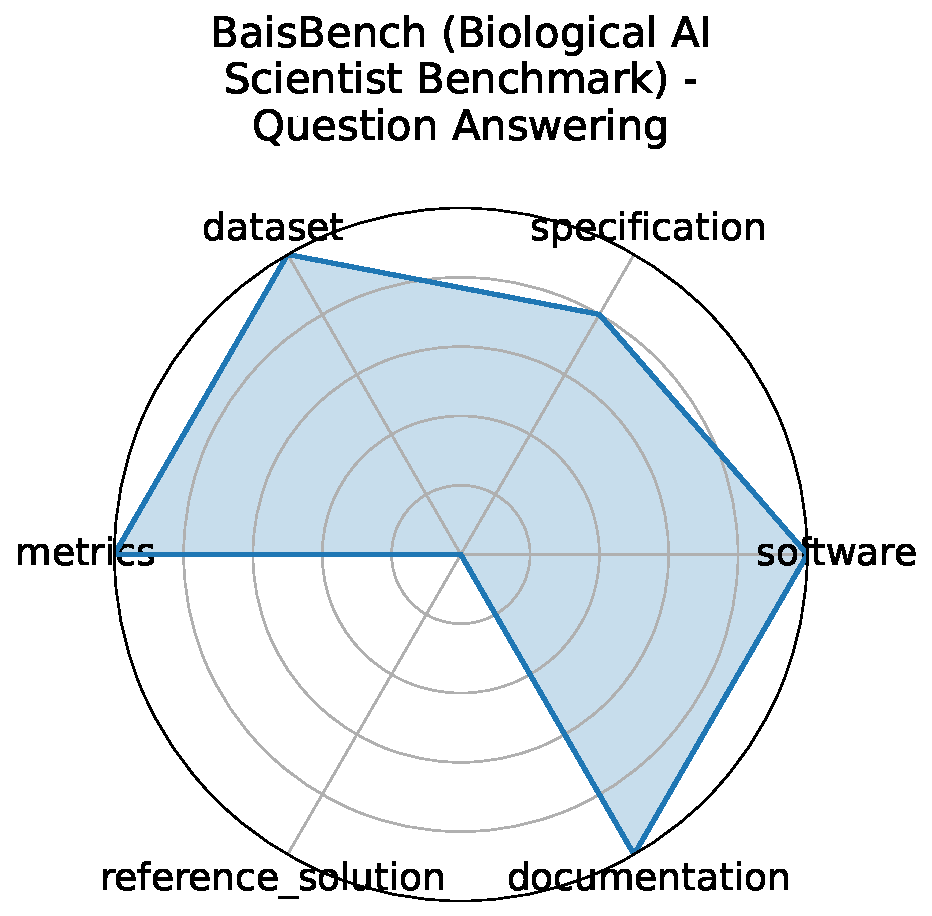
\includegraphics[width=0.2\textwidth]{baisbench_biological_ai_scientist_benchmark_-_question_answering_radar.pdf}
}}
\clearpage